\section{Result and Discussion}
This section will discuss the experimental results of YOLOv8 and YOLOv10 on the proposed khmer traffic sign dataset.
The results are compared across 20, 30 and 40 training epoch to analyze the effect of training for both models.
\subsection{Overall Model Performance}
\begin{table*}[t]
    \centering
    \caption{Performance comparison of YOLOv8 and YOLOv10 at different training epochs.}
    \label{tab:model_performance}
    \begin{tabular}{llccccc}
        \hline\hline
        Model & Epoch & Precision (\%) & Recall (\%) & F1-Score (\%) 
        & mAP@50 (\%) & mAP@50-95 (\%) \\
        \hline
        YOLOv8  & 20 & 94.54 & 95.81 & 95.17 & 97.58 & 76.70 \\
        YOLOv8  & 30 & 95.92 & 95.27 & 95.59 & 97.99 & 77.32 \\
        \textbf{YOLOv8}  & \textbf{40} & \textbf{96.58} & \textbf{95.28} & \textbf{95.93} 
                 & \textbf{98.18} & \textbf{77.53} \\
        \hline
        YOLOv10 & 20 & 93.86 & 94.16 & 94.01 & 97.14 & 76.83 \\
        YOLOv10 & 30 & 95.61 & 94.69 & 95.14 & 97.64 & 77.39 \\
        YOLOv10 & 40 & 95.64 & 95.18 & 95.41 & 97.98 & \textbf{77.79} \\
        \hline\hline
    \end{tabular}
\end{table*}
Table 3 presents the performance of YOLOv8 and YOLOv10 at 20, 30, and 40 training epochs using Precision, Recall, F1-Score, mAP@50, and mAP@50-95. Both models achieved high detection performance. YOLOv8 obtained the highest Precision (96.58\%), F1-Score (95.28\%), and mAP@50 (98.18\%), while YOLOv10 achieved the highest mAP@50-95 (77.79\%). Overall, both models performed similarly well on the Khmer traffic sign dataset.

The outcomes of different training epochs on the performance of YOLOv8 and YOLOv10 is demonstrate in Figure \ref{fig:mAP50_comparison}. For YOLOv8, mAP@50 increased from 97.58\% at 20 epochs
to 97.99\% at 30 epochs and reached 98.18\% at 40 epochs. Furthermore, the mAP@50-95 improved from 76.70\% to 77.32\% and reached 77.53\%.
YOLOv10 also showed a consistent performance, with mAP@50 increasing from 97.14\% at 20 epochs to 97.64\% at 30 epochs and 97.98\% at 40 epochs. Additionally, 
mAP@50-95 also increased from 76.83\% to 77.39\% and 77.79\%, as represent in Table \ref{tab:model_performance}.  

These results indicate that increasing the training epochs from 20 to 40 improved both models, while performance increase gradually become smaller, indicating stable performance.
\begin{figure}[ht]
    \centering
    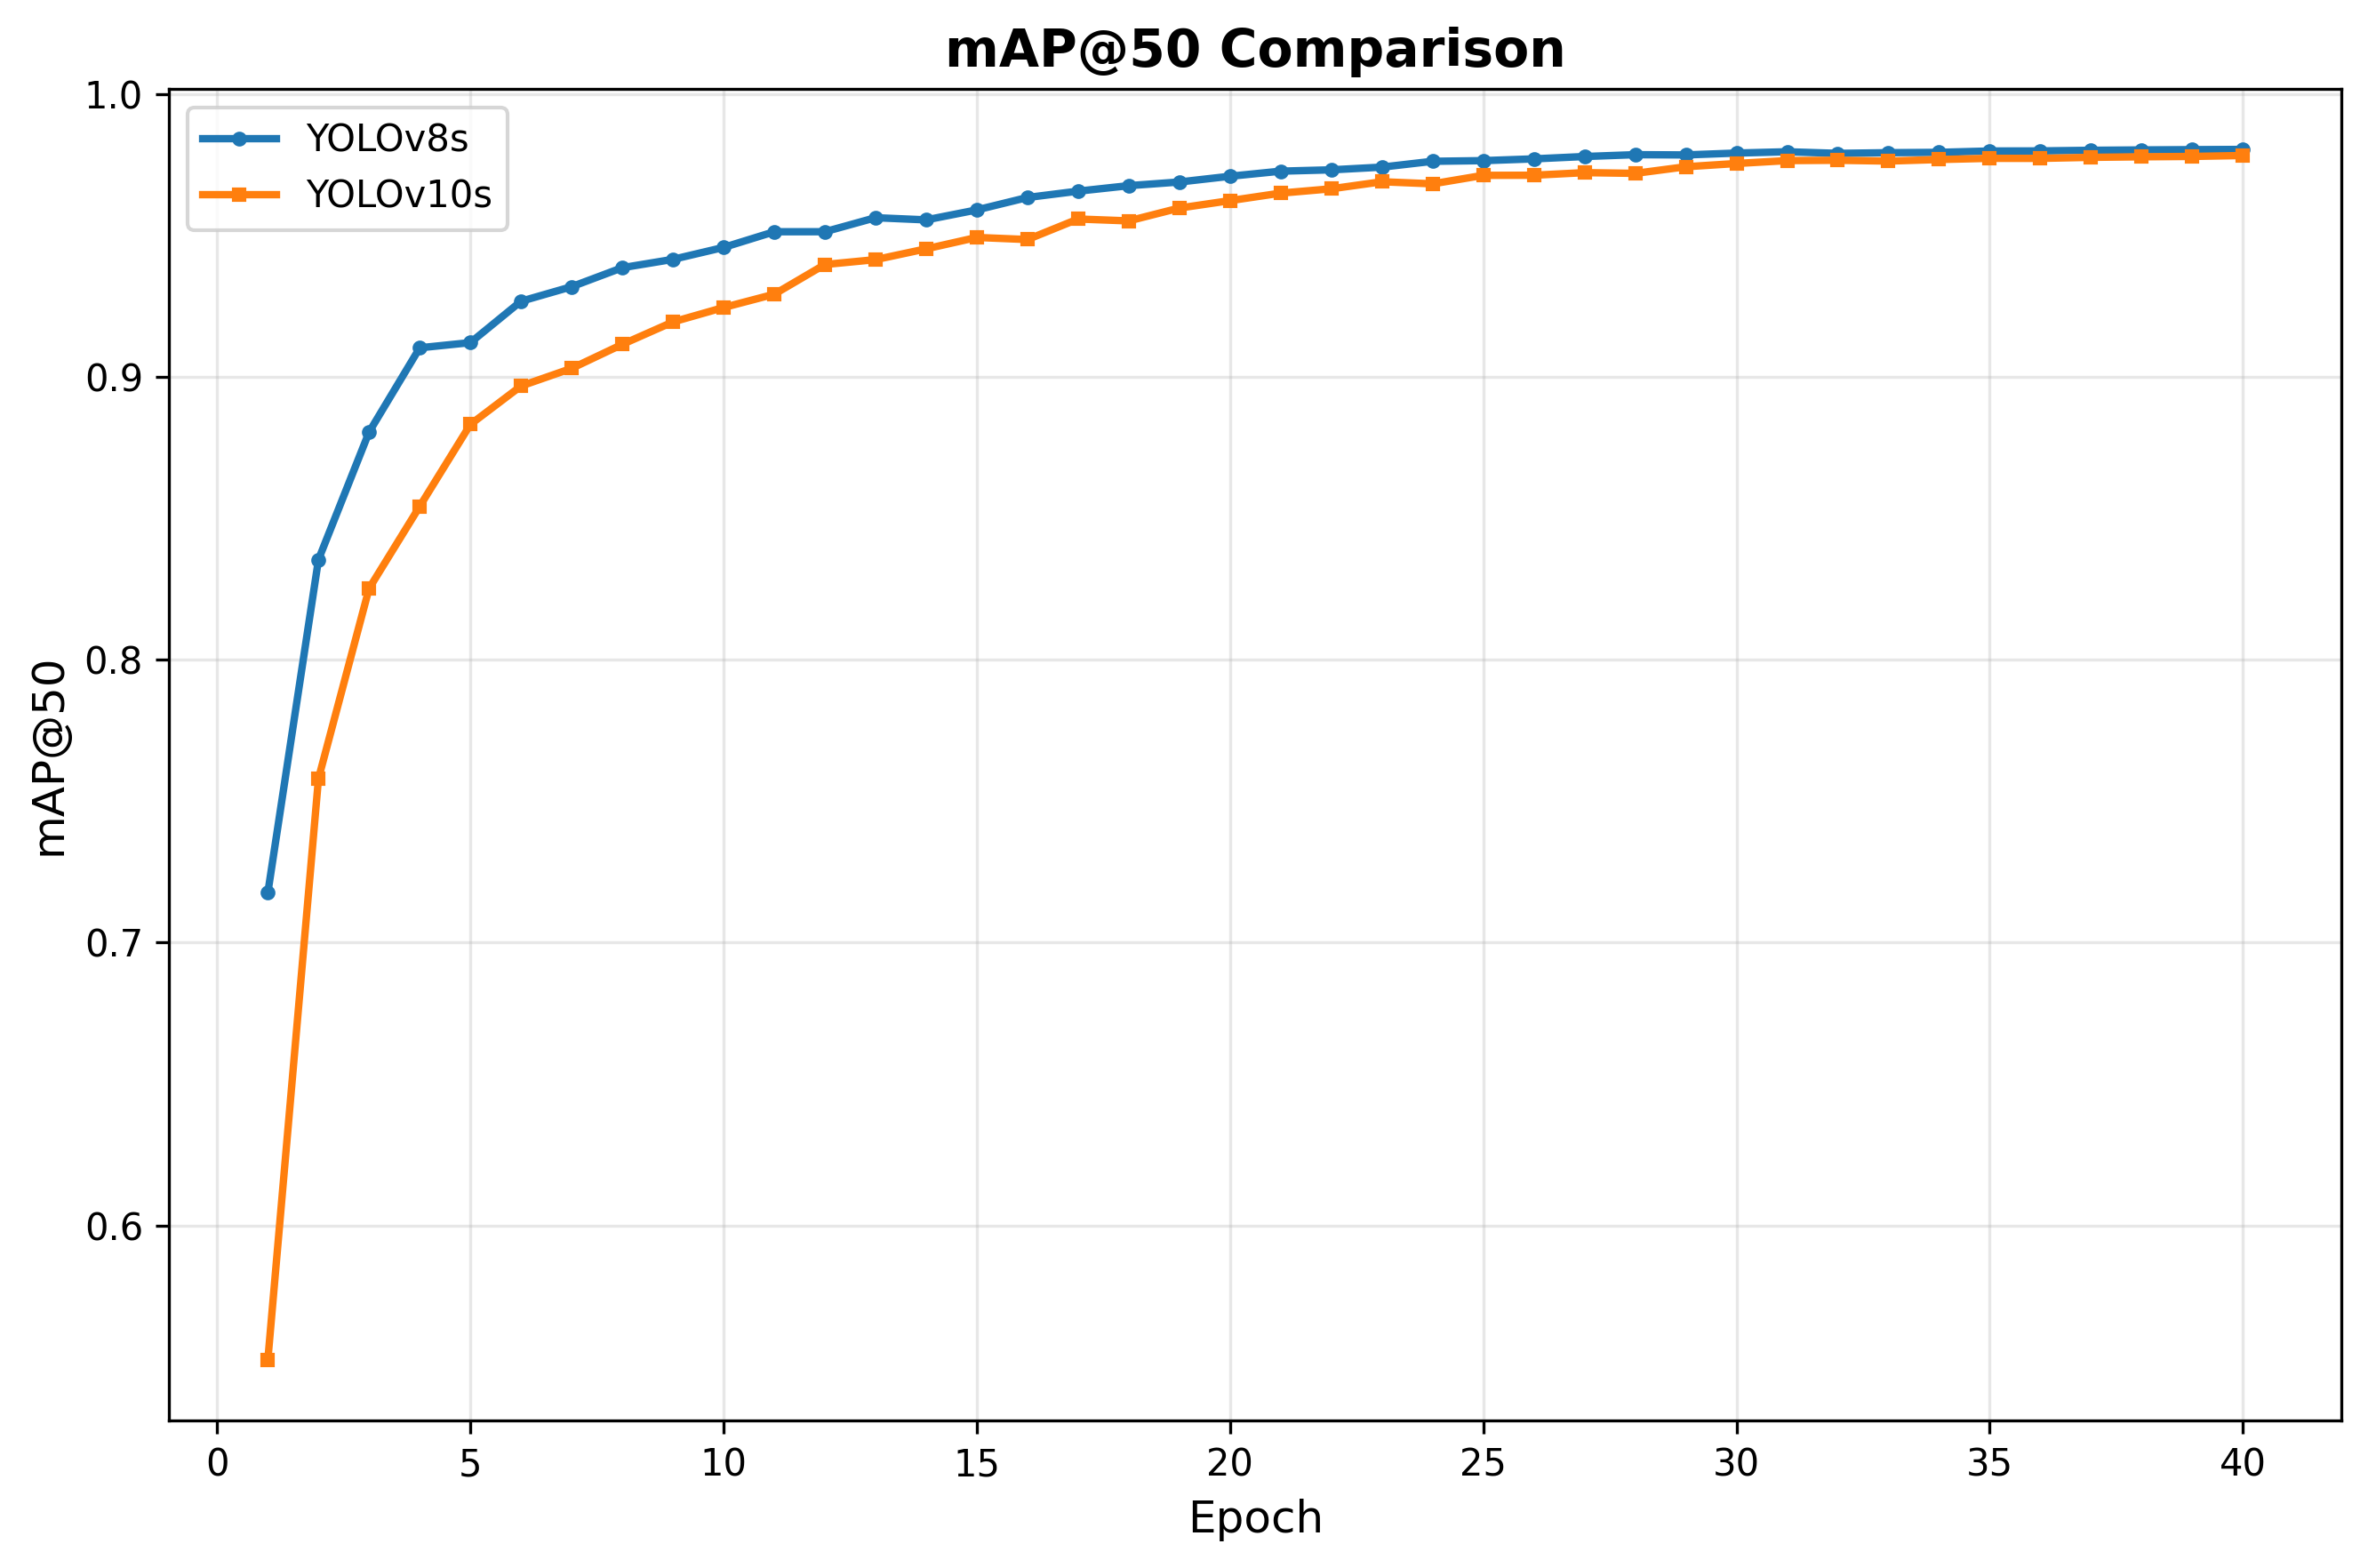
\includegraphics[width=\columnwidth]{./fig/comparison_mAP50.png}
    \caption{mAP@50 learning curves for YOLOv8s and YOLOv10s across 40 epochs.}
    \label{fig:mAP50_comparison}
\end{figure}
\subsection{Performance Evaluation of YOLOv8 and YOLOv10}
As shown in Table \ref{tab:model_performance}, YOLOv8 demonstrated slightly stronger overall performance than YOLOv10 on the Khmer traffic sign dataset. YOLOv8 achieved stronger results across most of the evaluated metrics, demonstrating its effectiveness in detection traffic signs.
However, YOLOv10 showed comparable performance and demonstrated a little advantage in mAP@50-95, indicate that YOLOv10 perform better under more stringent IoU thresholds.
Overall, although the performance difference between the two models was slightly small, YOLOv8 proved a little advantage and can therefore be considered the better performance model for proposed dataset. 
\subsection{Detection Performance Analysis}
Figure \ref{fig:qualitative_detection_performance} demonstrates the detection and classification results generated by the selected YOLOv8 model under different conditions. The model successfully detected and classified traffic signs, these results also show that the model
can recognize small or distant traffic signs and provide reliable predictions under challenging conditions, including bright lighting, low lighting and blurred images. These results provide further evidence of the model's detection capability

\begin{figure}[ht]
    \centering
    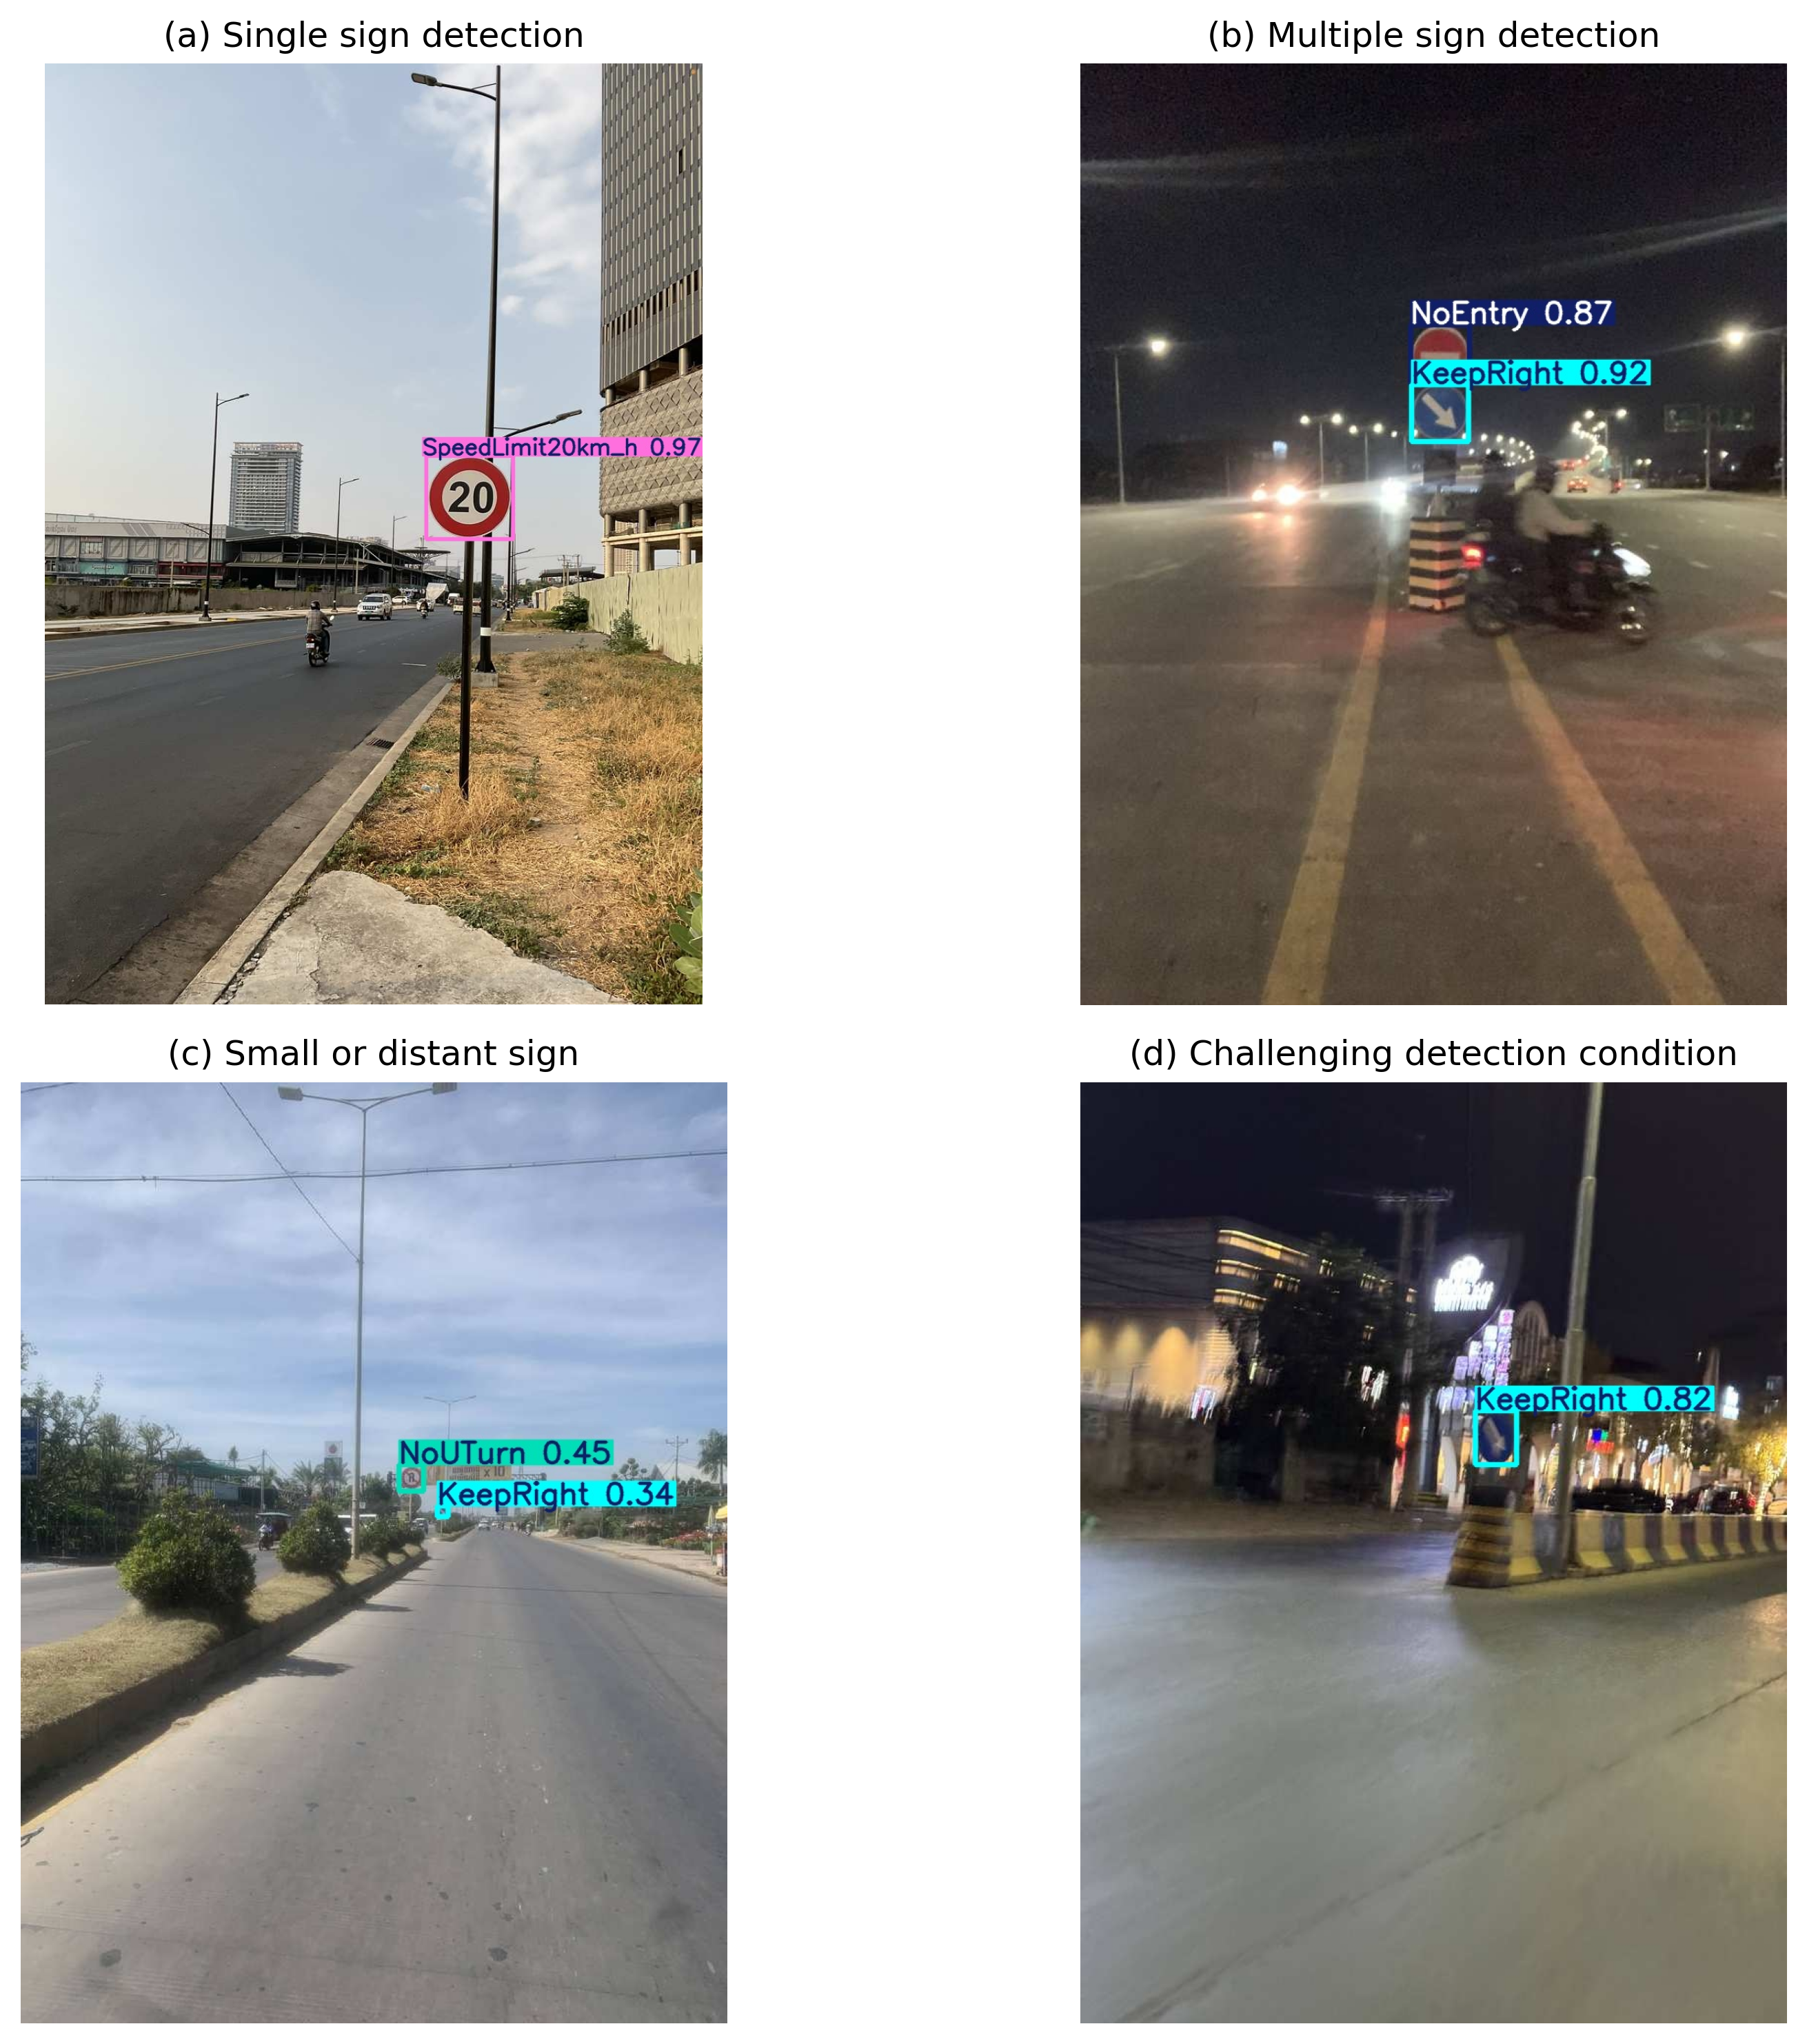
\includegraphics[width=\columnwidth]{./fig/qualitative_detection_results.png}
    \caption{Qualitative detection results of YOLOv8 under different conditions: (a) single traffic sign, (b) multiple traffic signs, (c) small or distant traffic sign, and (d) challenging detection condition.}
    \label{fig:qualitative_detection_performance}
\end{figure}
